\subsection{System modelling }
This section describes the interconnected component in a water distributed network (WDN) using Graph Theory. Furthermore thee component classes will be examined, ie. pipes, pumps and valves.


\subsection{Graph Theory}
When using graph theory as an analytical tool the incident matrix $H$ comes in handy when describing the connection between edges and nodes. The $H$ matrix is defined as follows: 

\subsubsection{The Incident Matrix}
\begin{equation}
	H_{i,j} = \begin{cases}
		-1 & \text{If the $j^{th}$ edge enters the $i^{th}$ node} \\
		0 & \text{If the $j^{th}$ edge is not connected to the $i^{th}$ node} \\
		1 & \text{If the $j^{th}$ edge s leaving the $i^{th}$ node}
	\end{cases}
\end{equation} %Description of the incident matrix

\subsubsection{Spanning Tree}
The spanning tree is the connected graph but with no loops, i.e you can not find a route around the graph where you start and end in the same node without entering a node more than one time. 
When adding one chord to the graph, exactly one loop is created.


\subsubsection{The Loop Marix}
The definition of a loop is a unique route along the edges of the graph network, where all nodes are unique except the end node - In a loop the end node must also be the start node.

The loop-matrix can be calculated in one of two ways. The first one is shown in the equation below

\begin{equation}\label{eq:LoopMatrix}
	B = \begin{bmatrix}
		I & -\bar{H}_{C}^{T}\cdot\bar{H}_{T}^{-T}
	\end{bmatrix}
\end{equation}


With $\bar{H}_{C}$ being the matrix containing only chord columns of the incident matrix. The same goes for  $\bar{H}_{T}$, containing only the non-chord columns. The bar indicates that the row corresponding to the reference node has been removed from the incident matrix.

The other method is more graphical but can be formulated as follows: 

Adding one chord to the spanning tree, creates exactly one loop. Writing up the edges in the loop, with signs corresponing to the incident matrix creates a row in the loop matrix $ B $. 


\newpage
\subsection{Simplified system}
\begin{figure}[h!]
	\centering
	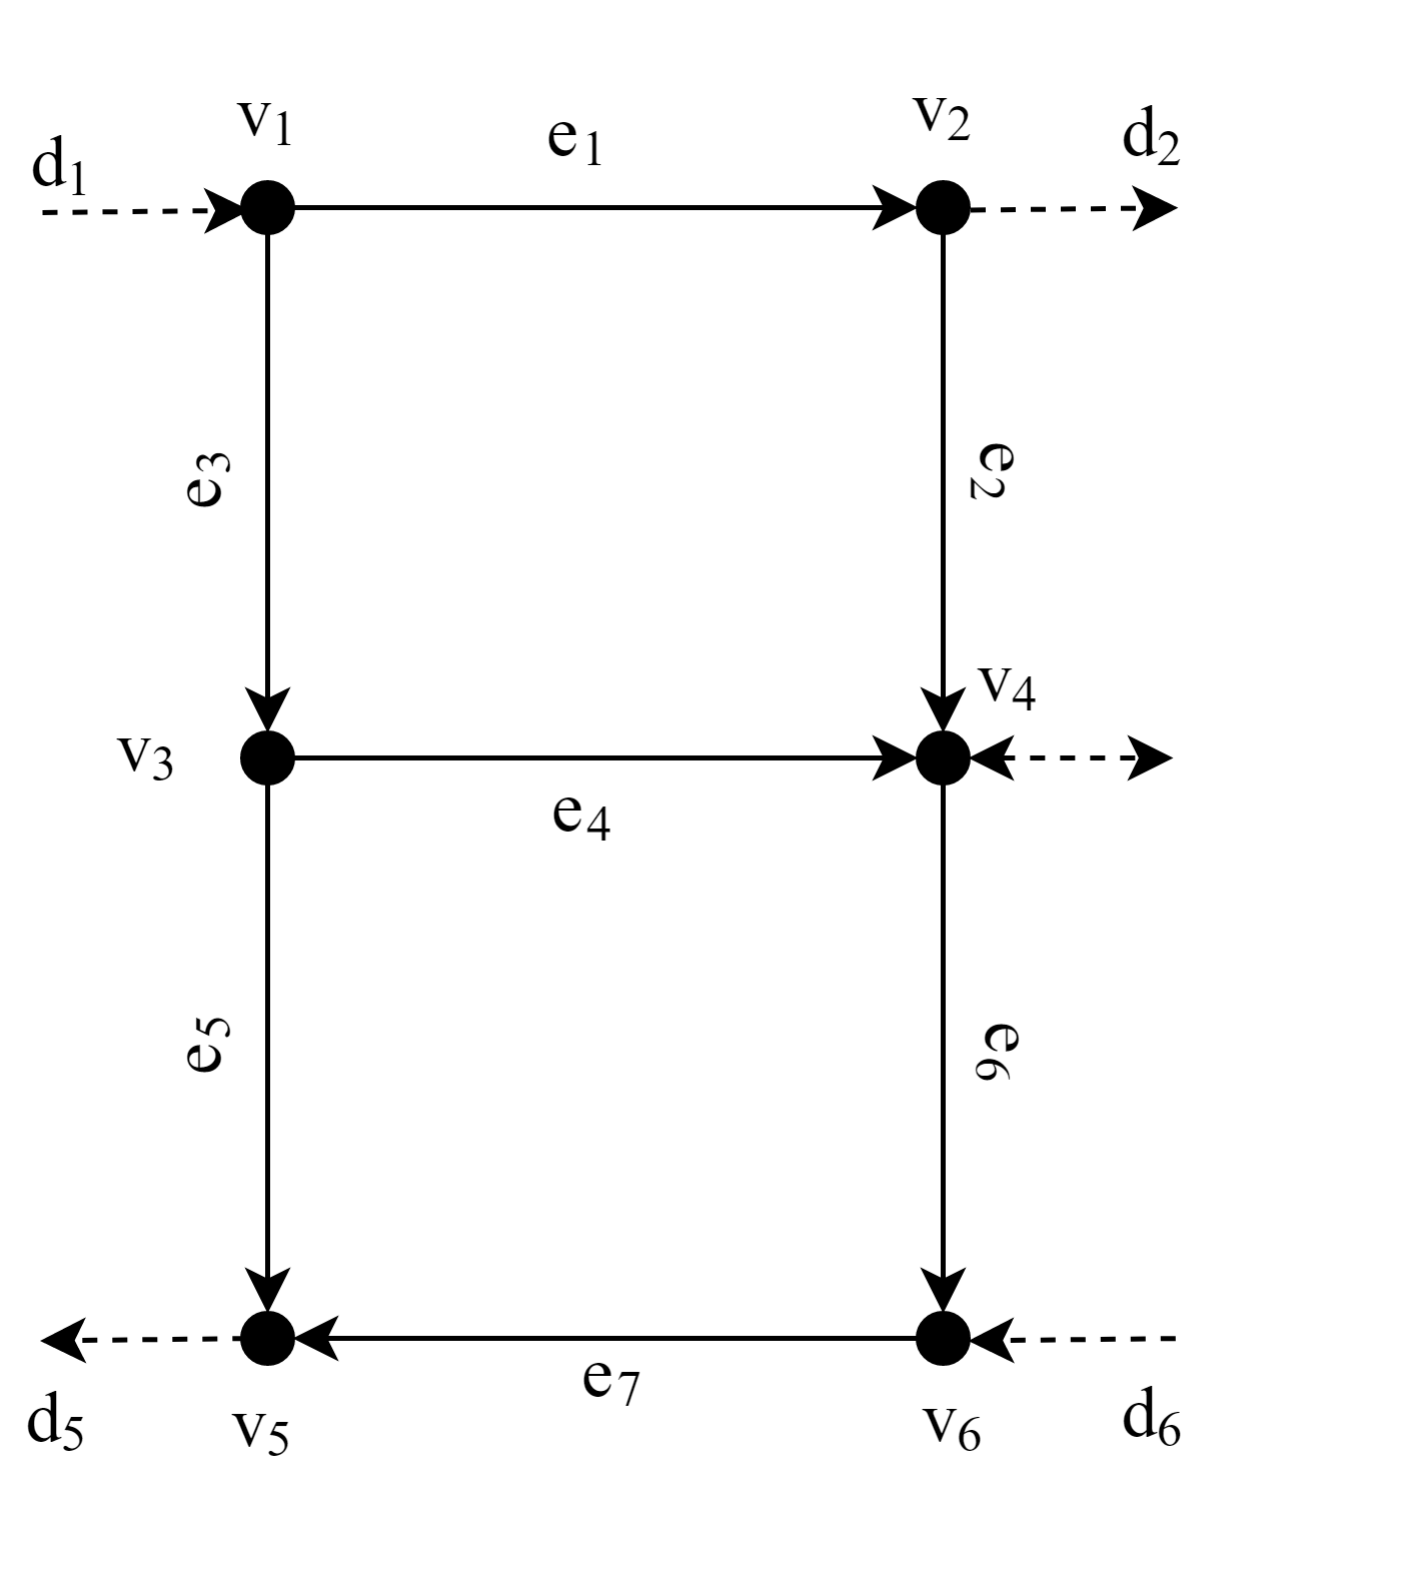
\includegraphics[width=0.5\textwidth]{Pictures/Graph.png}
	\caption{Graph of simplified WDN network \cite{Rathore930}}
	\label{fig:graph}
\end{figure}

When applying the rules shown above for the simplified graph model of the WDN the incident matrix in \cref{eq:H_simplified}.

\begin{equation}
	H = \begin{bmatrix}
		1 & 0 & 1 & 0 & 0 & 0 & 0\\
		-1 & 1 & 0 & 0 & 0 & 0 & 0\\
		0 & 0 & -1 & 1 & 1 & 0 & 0\\
		0 & -1 & 0 & -1 & 0 & 1 & 0\\
		0 & 0 & 0 & 0 & -1 &  0  & -1\\
		0 & 0 & 0 & 0 & 0 & -1 & 1
	\end{bmatrix}
	\label{eq:H_simplified}
\end{equation} %The incident matrix for system


The reduced incident matrix by taking an arbitrary vertex as a reference, and removing that vertex-row from \cref{eq:H_simplified}. We chose the $4^{th}$ vertex, which results in the following reduced incident matrix:
\begin{equation}
	\bar{H} = \begin{bmatrix}
		1 & 0 & 1 & 0 & 0 & 0 & 0\\
		-1 & 1 & 0 & 0 & 0 & 0 & 0\\
		0 & 0 & -1 & 1 & 1 & 0 & 0\\
		0 & 0 & 0 & 0 & -1 &  0  & -1\\
		0 & 0 & 0 & 0 & 0 & -1 & 1
	\end{bmatrix}
\end{equation}

Chords and edges of the spanning tree

\begin{equation} 
	\begin{split}
		E_{C} &= \{e_{1},e_{4}\}   \\ E_{T} &= \{e_2,e_3,e_5,e_6,e_7\}
	\end{split}
\end{equation}


\begin{equation}
	B = \begin{bmatrix}
		1 & 0 & 1 & -1 & -1 & 1 & 1\\
		0 & 1 & 0 & 0 & -1 & 1 & 1\\
	\end{bmatrix}
\end{equation}
\newpage

\subsection{Detailed system}
In this section we present a graph of the water distribution network.

\begin{figure}[h]
	\centering
	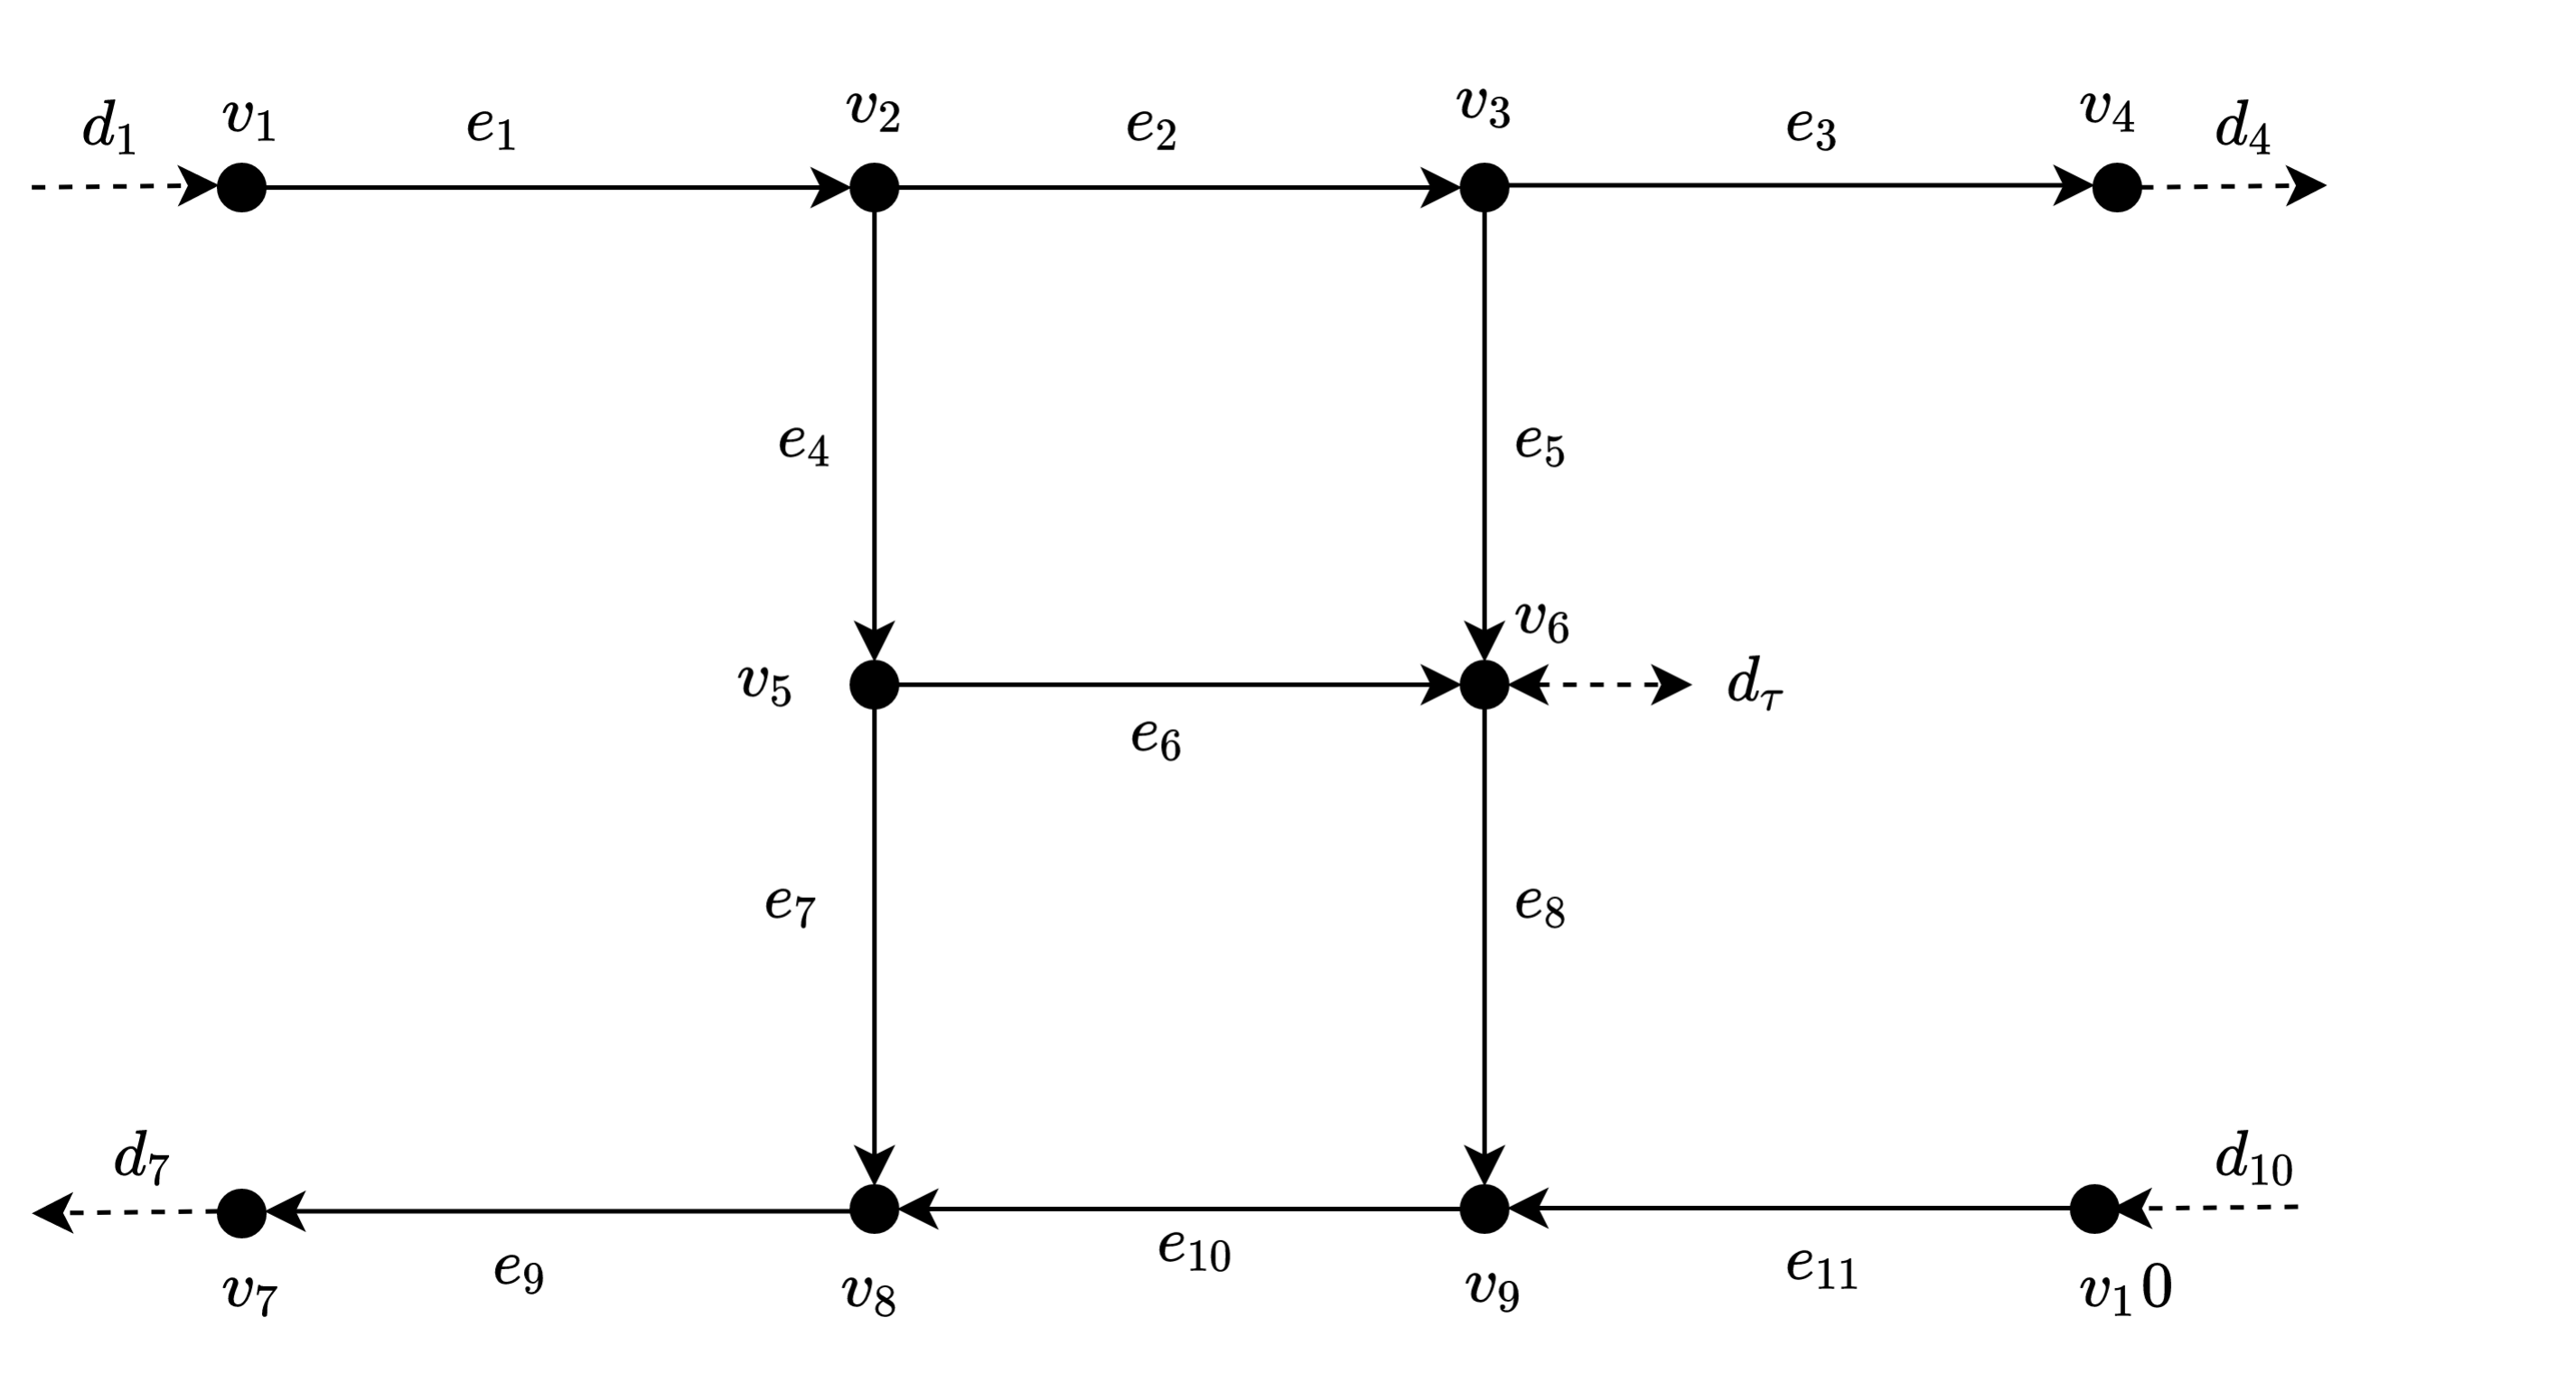
\includegraphics[width=0.7\textwidth]{Pictures/GraphDetailed.png}
	\caption{Detailed graph model of WDN} 
		\label{fig:WDNDetailed}
	\end{figure}
$ d_1 $ and $ d_{10} $ represent the waterflow into the system from the pumps, which are represented by edge $ e_1 $ and $ e_{11} $ respectively.
$ d_4 $ and $ d_7 $ represent the waterflow out of the system from the valves, which are represented by edge $ e_3 $ and $ e_9 $ respectively.
$ d_\tau $ represent the waterflow in an out of the tank.
The incident matrix for the graph on \cref{fig:WDNDetailed} is shown blow in \cref{eq:H_detailed}.
	
	\begin{equation}\label{eq:H_detailed}
		H = \kbordermatrix{
		& e_1 & e_2 & e_3   & e_4  & e_5 & e_6  & e_7  & e_8  & e_9  & e_{10}  & e_{11}  \\	
		v_1& 1 & 0 & 0   & 0  & 0  & 0  & 0  & 0  & 0  & 0  & 0 \\
		v_2& -1 & 1 & 0  & 1  & 0  & 0  & 0  & 0  & 0  & 0  & 0 \\
		v_3& 0 & -1 & 1  & 0  & 1  & 0  & 0  & 0  & 0  & 0  & 0 \\
		v_4& 0 & 0  & -1 & 0  & 0  & 0  & 0  & 0  & 0  & 0  & 0 \\
		v_5& 0 & 0  & 0  & -1 & 0  & 1  & 1  & 0  & 0  & 0  & 0 \\
		v_6&0 & 0  & 0  & 0  & -1 & -1 & 0  & 1  & 0  & 0  & 0 \\
		v_7& 0 & 0  & 0  & 0  & 0  & 0  & 0  & 0  & -1 & 0  & 0 \\
		v_8& 0 & 0  & 0  & 0  & 0  & 0  & -1 & 0  & 1  & -1 & 0 \\
		v_9& 0 & 0  & 0  & 0  & 0  & 0  & 0  & -1 & 0  & 1  & -1 \\
		v_{10}& 0 & 0  & 0  & 0  & 0  & 0  & 0  & 0  & 0  & 0  & 1 \\
	}
	\end{equation}	
	
The chords and the spanning tree is chosen from \cref{fig:WDNDetailed} \footnote{Note that you can obtain several spanning trees in this network, just by choosing different chords}
	
\begin{equation*} 
	\begin{split}
		E_{C} &= \{e_{2},e_{6}\}   \\ E_{T} &= \{e_1,e_3,e_4,e_5,e_7, e_8, e_9, e_{10} , e_{11}\}
	\end{split}
\end{equation*}	
	
	By choosing the xxx node as a reference, and removing it from the incident matrix we obtain:
	\begin{equation}
		\bar{H} = \kbordermatrix{
		& e_1 & e_2 & e_3   & e_4  & e_5 & e_6  & e_7  & e_8  & e_9  & e_{10}  & e_{11}  \\	
		v_1& 1 & 0 & 0   & 0  & 0  & 0  & 0  & 0  & 0  & 0  & 0 \\
		v_2& -1 & 1 & 0  & 1  & 0  & 0  & 0  & 0  & 0  & 0  & 0 \\
		v_3& 0 & -1 & 1  & 0  & 1  & 0  & 0  & 0  & 0  & 0  & 0 \\
		v_4& 0 & 0  & -1 & 0  & 0  & 0  & 0  & 0  & 0  & 0  & 0 \\
		v_5& 0 & 0  & 0  & -1 & 0  & 1  & 1  & 0  & 0  & 0  & 0 \\
		v_7& 0 & 0  & 0  & 0  & 0  & 0  & 0  & 0  & -1 & 0  & 0 \\
		v_8& 0 & 0  & 0  & 0  & 0  & 0  & -1 & 0  & 1  & -1 & 0 \\
		v_9& 0 & 0  & 0  & 0  & 0  & 0  & 0  & -1 & 0  & 1  & -1 \\
		v_{10}& 0 & 0  & 0  & 0  & 0  & 0  & 0  & 0  & 0  & 0  & 1 \\
		}
	\end{equation}
	
Furthermore we can define the open-node matrix $F$ and tank matrix $G$:
	
	\begin{equation}\label{eq:ONandTankMatrix}
		F = \kbordermatrix{
			&d_{f_1}&d_{f_2}&d_{f_3}&d_{f_4}\\
		d_1	& 1 & 0 & 0 & 0\\
		d_2	& 0 & 0 & 0 & 0\\
		d_3 & 0 & 0 & 0 & 0\\
		d_4 & 0 & 1 & 0 & 0\\
		d_5 & 0 & 0 & 0 & 0\\
		d_6 & 0 & 0 & 0 & 0\\
		d_7 & 0 & 0 & 1 & 0\\
		d_8 & 0 & 0 & 0 & 0\\
		d_9 & 0 & 0 & 0 & 0\\
		d_{10}& 0 & 0 & 0 & 1 \\
			},
	\qquad
		G = \kbordermatrix{
			&d_{\tau_1}\\
			d_1& 0\\
			d_2& 0\\
			d_3& 0\\
			d_4& 0\\
			d_5& 0\\
			d_6& 1\\
			d_7& 0\\
			d_8& 0\\
			d_9& 0\\
			d_{10}& 0 \\
			}
	\end{equation}

with their reference-respective equivalents given by:

\begin{equation}\label{eq:FbarGbar}
	\bar{F} = F \setminus F_{6\star} \wedge \bar{G} = G \setminus G_{6\star}
\end{equation}

where the notation $X_{6\star}$ denotes the entire 6th row\footnote{Correspondingly, $X_{\star6}$ would denote the entire 6th column} of the matrix $X$ and $\setminus$ is the set relative complement operator. These matrices map demands at their respective nodes into the vector of total demands in the system $d \vee \bar{d}$.

\subsection{Detailed system V2}

The H matrix:

$ H = \begin{bmatrix}
	1	& 0 	& 0 	& 0 	& 0 	& 0 	& 0 	& 0 	& 0 	& 0 	& 0 	& 0 	& 0 	& 0 \\
	-1	& 1 	& 0 	& 0 	& 0 	& 0 	& 0 	& 0 	& 0 	& 0 	& 0 	& 0 	& 0 	& 0 \\
	0	& -1 	& 1 	& 0 	& 1 	& 0 	& 0 	& 0 	& 0 	& 0 	& 0 	& 0 	& 0 	& 0 \\
	0	& 0 	& -1 	& 1 	& 0 	& 1 	& 0 	& 0 	& 0 	& 0 	& 0 	& 0 	& 0 	& 0 \\
	0	& 0 	& 0 	& -1 	& 0 	& 0 	& 0 	& 0 	& 0 	& 0 	& 0 	& 0 	& 0 	& 0 \\
	0	& 0 	& 0 	& 0 	& -1 	& 0 	& 1 	& 1 	& 0 	& 0 	& 0 	& 0 	& 0 	& 0 \\
	0	& 0 	& 0 	& 0 	& 0 	& -1 	& -1 	& 0 	& 1 	& 0 	& 0 	& 0 	& 0 	& 0 \\
	0	& 0 	& 0 	& 0 	& 0 	& 0 	& 0 	& 0 	& -1 	& 1 	& 0 	& 0 	& 0 	& 0 \\
	0	& 0 	& 0 	& 0 	& 0 	& 0 	& 0 	& 0 	& 0 	& 0 	& -1 	& 0 	& 0 	& 0 \\
	0	& 0 	& 0 	& 0 	& 0 	& 0 	& 0 	& -1 	& 0 	& 0 	& 1 	& -1 	& 0 	& 0 \\
	0	& 0 	& 0 	& 0 	& 0 	& 0 	& 0 	& 0 	& 0 	& -1 	& 0 	& 1 	& -1 	& 0 \\
	0	& 0 	& 0 	& 0 	& 0 	& 0 	& 0 	& 0 	& 0 	& 0 	& 0 	& 0 	& 1 	& -1\\
	0	& 0 	& 0 	& 0 	& 0 	& 0 	& 0 	& 0 	& 0 	& 0 	& 0 	& 0 	& 0 	& 1    
\end{bmatrix}  $

The H\_bar matrix:

$ \bar{H} = \begin{bmatrix}
	1	& 0 	& 0 	& 0 	& 0 	& 0 	& 0 	& 0 	& 0 	& 0 	& 0 	& 0 	& 0 	& 0 \\
	-1	& 1 	& 0 	& 0 	& 0 	& 0 	& 0 	& 0 	& 0 	& 0 	& 0 	& 0 	& 0 	& 0 \\
	0	& -1 	& 1 	& 0 	& 1 	& 0 	& 0 	& 0 	& 0 	& 0 	& 0 	& 0 	& 0 	& 0 \\
	0	& 0 	& -1 	& 1 	& 0 	& 1 	& 0 	& 0 	& 0 	& 0 	& 0 	& 0 	& 0 	& 0 \\
	0	& 0 	& 0 	& -1 	& 0 	& 0 	& 0 	& 0 	& 0 	& 0 	& 0 	& 0 	& 0 	& 0 \\
	0	& 0 	& 0 	& 0 	& -1 	& 0 	& 1 	& 1 	& 0 	& 0 	& 0 	& 0 	& 0 	& 0 \\
	0	& 0 	& 0 	& 0 	& 0 	& -1 	& -1 	& 0 	& 1 	& 0 	& 0 	& 0 	& 0 	& 0 \\
	0	& 0 	& 0 	& 0 	& 0 	& 0 	& 0 	& 0 	& -1 	& 1 	& 0 	& 0 	& 0 	& 0 \\
	0	& 0 	& 0 	& 0 	& 0 	& 0 	& 0 	& 0 	& 0 	& 0 	& -1 	& 0 	& 0 	& 0 \\
	0	& 0 	& 0 	& 0 	& 0 	& 0 	& 0 	& -1 	& 0 	& 0 	& 1 	& -1 	& 0 	& 0 \\
	0	& 0 	& 0 	& 0 	& 0 	& 0 	& 0 	& 0 	& 0 	& -1 	& 0 	& 1 	& -1 	& 0 \\
	0	& 0 	& 0 	& 0 	& 0 	& 0 	& 0 	& 0 	& 0 	& 0 	& 0 	& 0 	& 1 	& -1\\
\end{bmatrix}  $

The B matrix (not even started):

$ B = \begin{bmatrix}
	1	& 0 	& 0 	& 0 	& 0 	& 0 	& 0 	& 0 	& 0 	& 0 	& 0 	& 0 \\
	-1	& 1 	& 0 	& 0 	& 0 	& 0 	& 0 	& 0 	& 0 	& 0 	& 0 	& 0 \\
\end{bmatrix}  $

